\paragraph{Returning}

To \emph{return} means to transfer back some value from the function to where it was called. Most programming languages use the keyword \emph{return} for this. The value that is returned is sometimes called the \emph{result} of the function. In the code where the function is called, the function call is replaced by its result in the same way that we use replace variable names with their respective values each time we calculate using variables.

\paragraph{Types}

Right at the start of this chapter we showed the following prototype of a function definition:

\begin{verbatim}
<type> <name of function>(<parameter list>):
  <function body>
\end{verbatim}

Up until now we have only used \texttt{void} for \texttt{<type>}. We can now define that \texttt{void} means that a function \emph{returns nothing}, meaning that the function will not contain a \texttt{return} statement.

Now if we would like to have the function return something, we will specify as \texttt{<type>} what kind of value the function will be returning. In this book, we will use the type \texttt{int}, \texttt{float} and \texttt{string}.

\paragraph{Tracing}

Functions that calculate and return something can be traced much like before. We add a \emph{back substitution} that fills in the returned value of the function into the place where it was called. Below, the function call \texttt{das(12)} returns the integer 3, which is then substituted into the \texttt{print} statement.

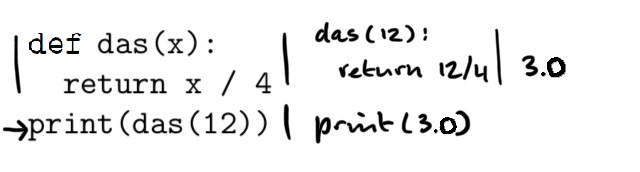
\includegraphics[width=.7\textwidth]{6-trace-returns.jpeg}
